\documentclass{article}
\usepackage{amsmath}
\usepackage{amssymb}
\usepackage{graphicx}
\usepackage{hyperref}
\usepackage[version=4]{mhchem}


\begin{document}
Let \(P\) be a point inside the square \(A B C D\). Find the area of the square if \(P A=5, P B=8\), and \(P C=13\).\\
(A) 153\\
(B) 126\\
(C) 128\\
(D) 130\\
(E) 132

Solution: (A).\\
Draw \(P E \perp A B, P F \perp B C\), as shown in the figure. Let the side length be \(a, P E=x\), and \(P F=y\).\\
\centering
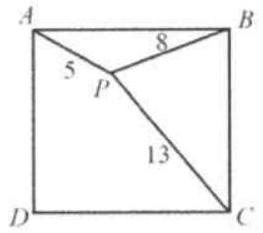
\includegraphics[width=\textwidth]{images/080(1).jpg}

Applying the Pythagorean Theorem on \(\triangle A E P, \triangle C P F\), and \(\triangle B P F\), we have

\[
\begin{aligned}
& x^{2}+(a-y)^{2}=25 \\
& (a-x)^{2}+y^{2}=169 \\
& x^{2}+y^{2}=64
\end{aligned}
\]

(1) - (3): \(a^{2}-2 a y=-39 \Rightarrow 4 a^{2} y^{2}=\left(a^{2}+39\right)^{2}\)\\
(2) - (3): \(a^{2}-2 a x=105 \Rightarrow 4 a^{2} x^{2}=\left(a^{2}-105\right)^{2}\)\\
\centering
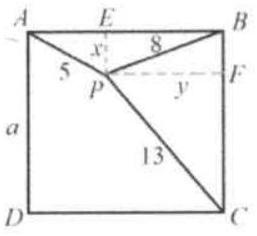
\includegraphics[width=\textwidth]{images/080(3).jpg}\\
(4) + (5): \(4 a^{2}\left(x^{2}+y^{2}\right)=\left(a^{2}+39\right)^{2}+\left(a^{2}-105\right)^{2}\)

Substituting (3) into (6): \(4 a^{2} \times 64=\left(a^{2}+39\right)^{2}+\left(a^{2}-105\right)^{2}\)\\
\(\Rightarrow \quad a^{4}-194 a^{2}-6273=0\).\\
So \(a^{2}=41\) or 153 .\\
Since \(P C<A C\), or \(13<\sqrt{2} a, 2 a^{2}>169\). Thus \(a^{2}=153\).\\
So the area is 153 .\\

\end{document}
